% !TEX root = ../../I4PRJ, Grp3 - Dokumentation.tex
\section{Web GUI}
Implementeringen af den grafiske brugergrænseflade til Web-applikationen beskrives i dette afsnit. Kildekoden ligger i Application.Web løsningen, hvori projektet af samme navn forefindes. Fælles for alle web views er, at de implementeret med HTML\todo{ordliste}. HTML er et markup language til hjemmesider. Hjemmesidens grafiske layout laves vha. CSS som beskriver, hvordan man vil have HTML vist på sin hjemmeside. Ydermere er der brugt javascript til fra client-side at kommunikerer med brugeren.Slutteligt er der brugt razor som er et server-side markup language. 

\subsection{LoginView}
LoginView ses på figuren nedenfor:

\begin{figure}
	\centering
	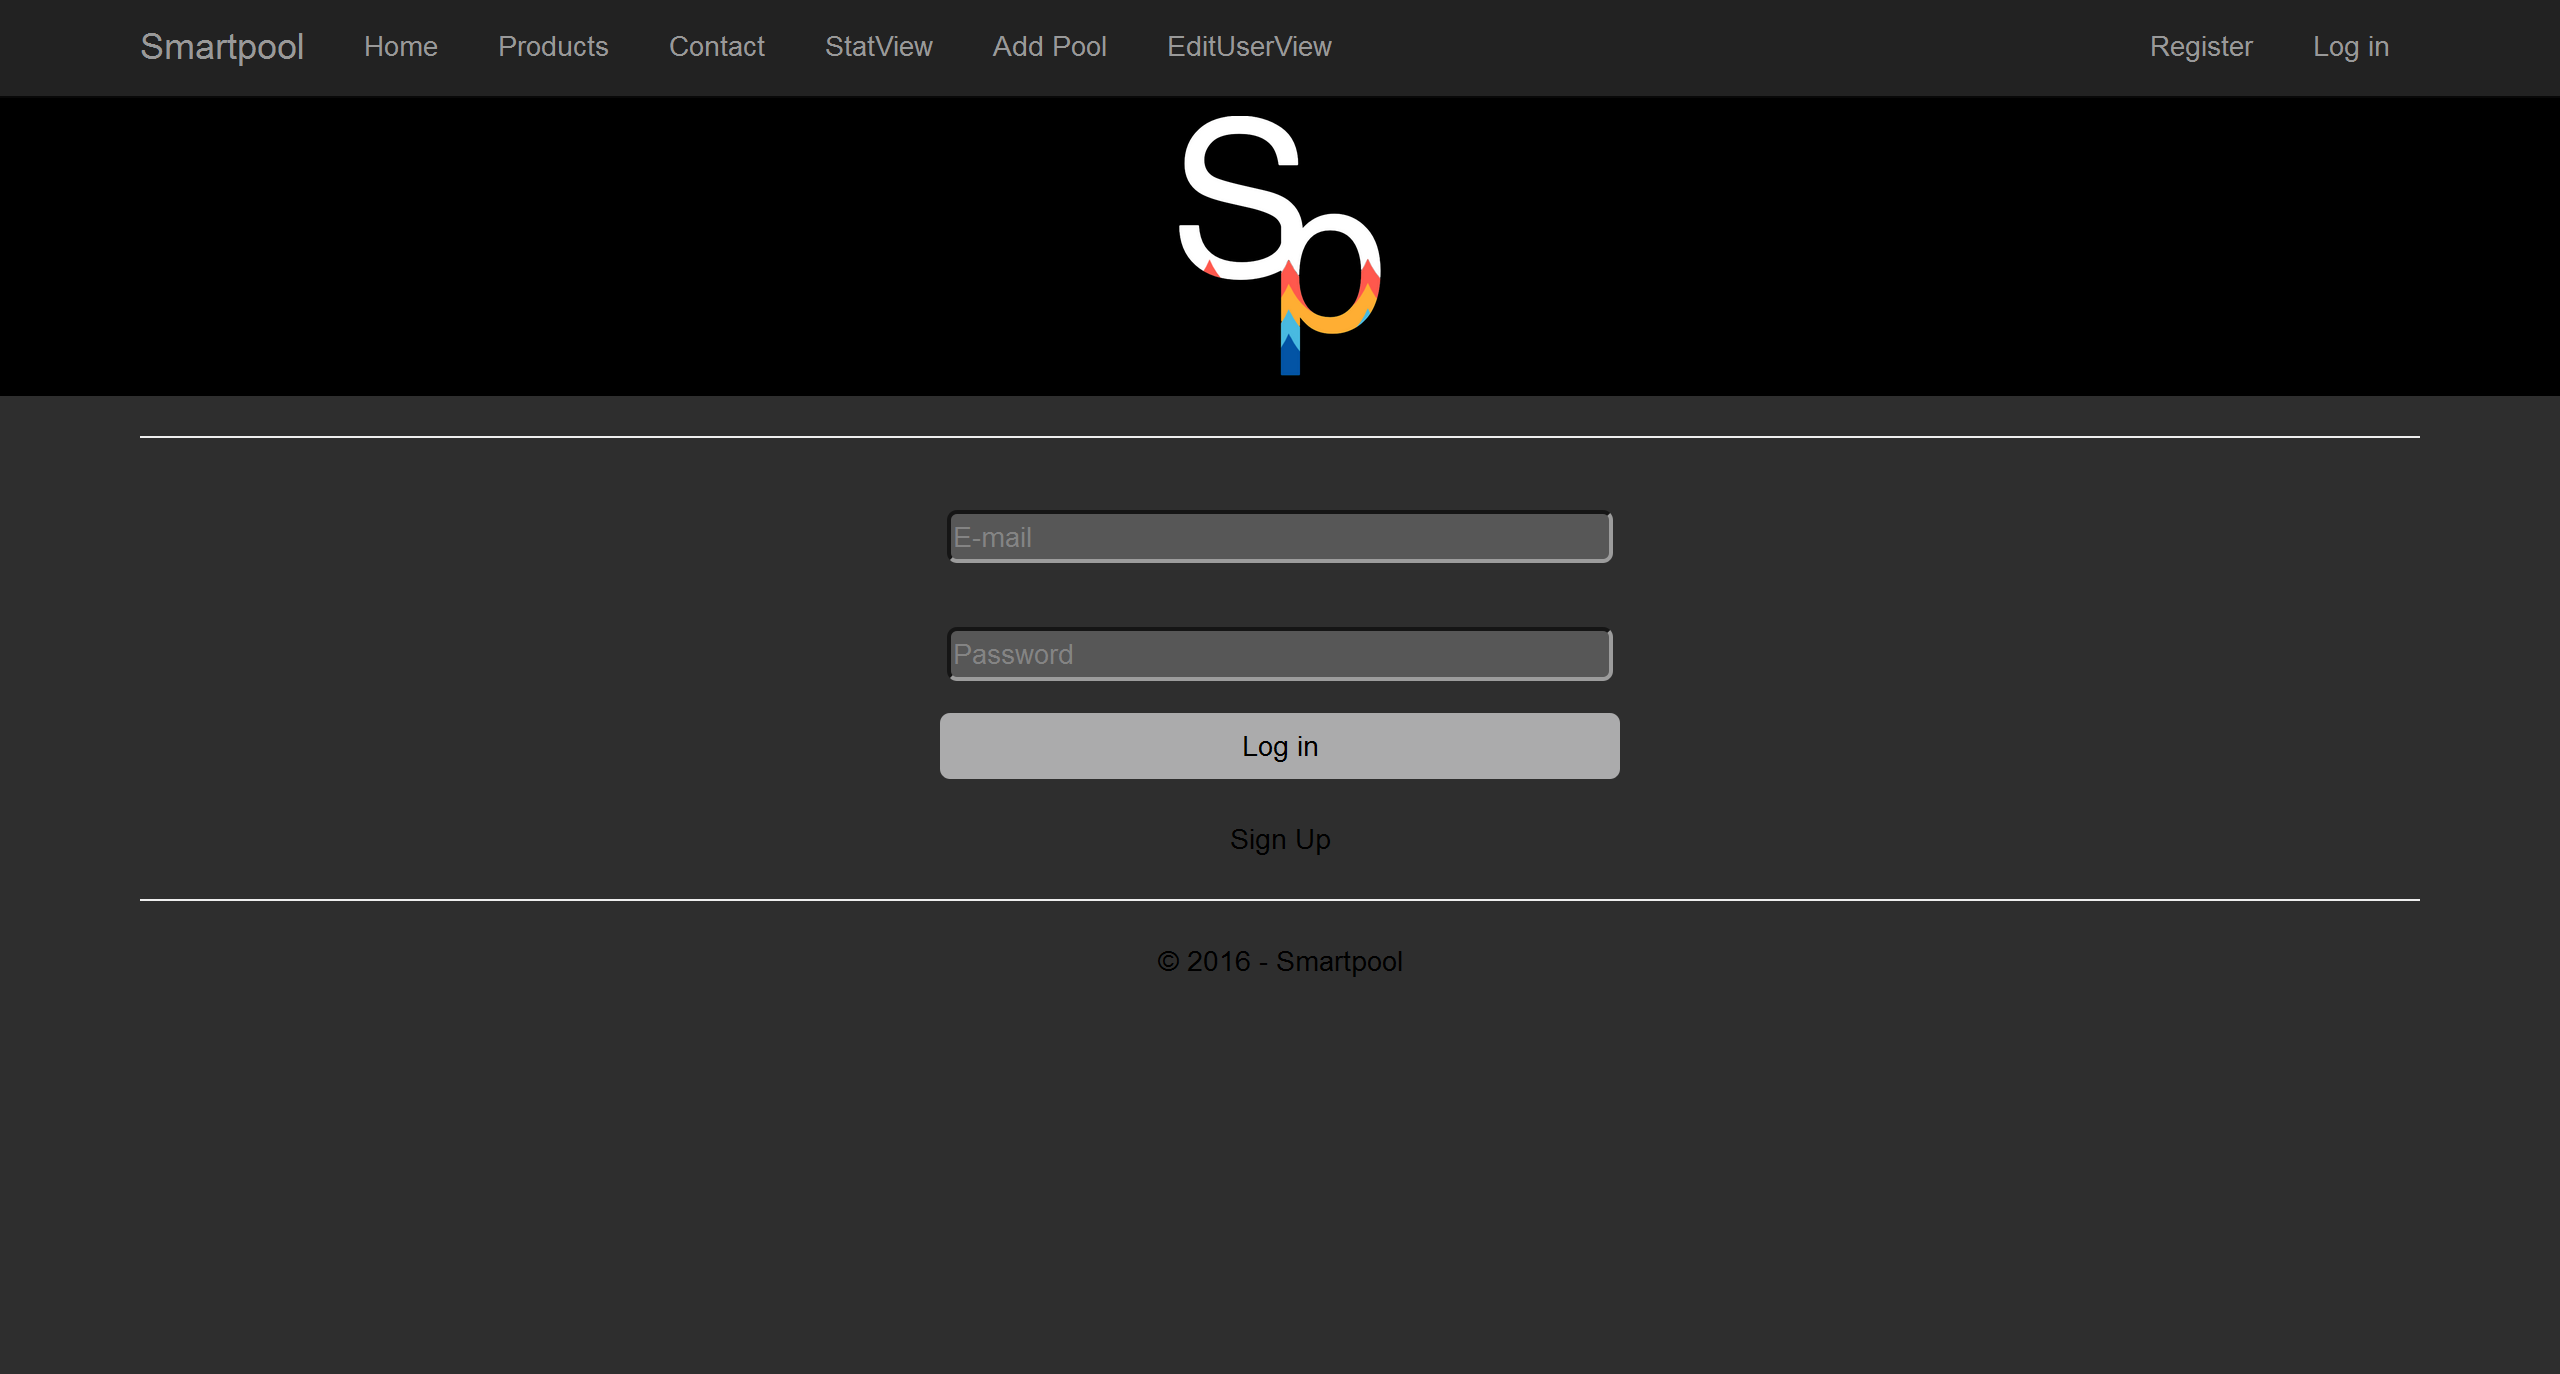
\includegraphics[width=1.0\linewidth]{figs/implementering/web_login}
	\caption{Web LoginView}
	\label{fig:webloginview}
\end{figure}

View grafikken er implementeret jævnfør det grafiske design. AccountController som implementerer ILoginView interfacet, har funktionen InitateController. Web-applikationens implementering af funktionen ses nedenfor:

\begin{lstlisting}[caption=InitiateController, label=code:InitaiteController]
private void InitiateController()
        {
            Controller = new LoginViewController(this, new ClientMessenger(new SynchronousSocketClient("93.166.226.201")));
            Controller.ViewDidLoad();
        }
\end{lstlisting} 

Funktionen oprtter en ny loginViewController, og giver den en ClientMessenger med sammen med en IP-adresse, hvorefter funktionen ViewDidLoad kaldes.

For at logge ind på serveren laves en 'Task' login.

\begin{lstlisting}[caption=Login, label=code:Login]
 // POST: /Account/Login
        [HttpPost]
        [AllowAnonymous]
        [ValidateAntiForgeryToken]
        public async Task<ActionResult> Login(LoginViewModel model, string returnUrl)
        {
            var loginController = Controller as ILoginViewController;
            loginController.DidChangeEmailText(model.Email);
            loginController.DidChangePasswordText(model.Password);
            loginController.ButtonPressed(LoginViewButton.LoginButton);

            _returnUrl = returnUrl;

            return View(model);
        }
\end{lstlisting} 

Funktionen sender request til server ved Button.Pressed. Funktionen LoginAccepted kaldes når serveren svarer tilbage.

\begin{lstlisting}[caption=LoginAccepted, label=code:LoginAccepted]
public void LoginAccepted()
        {
            ActionInvoker.InvokeAction(ControllerContext, "RedirectLogin");
        }
\end{lstlisting}

LoginAccepted 'Invoker' et ActionResult RedirectLogin.
 
 \begin{lstlisting}[caption=Redirect Login, label=code:redirectlogin]

        [AllowAnonymous]
        public ActionResult RedirectLogin()
        {
            return RedirectToLocal(_returnUrl);
        }
        }
\end{lstlisting}

RedirectLogin redirects til en anden side på serveren når login accepteres.

Ved forsøg på login, ses følgende på serveren:

\begin{figure}
	\centering
	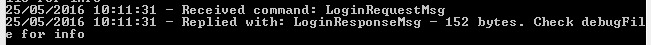
\includegraphics[width=1.0\linewidth]{figs/implementering/webtest}
	\caption{Web login forsøg}
	\label{fig:weblogintry}
\end{figure}

Testen bekræfter, at den generelle arkitektur for systemet virker sammen med ASP.NET MVC arkitekturen. 
 
\subsection{SignUpView}\label{sec: signupview}
SignUpView ses på figuren nedenfor:

\begin{figure}
	\centering
	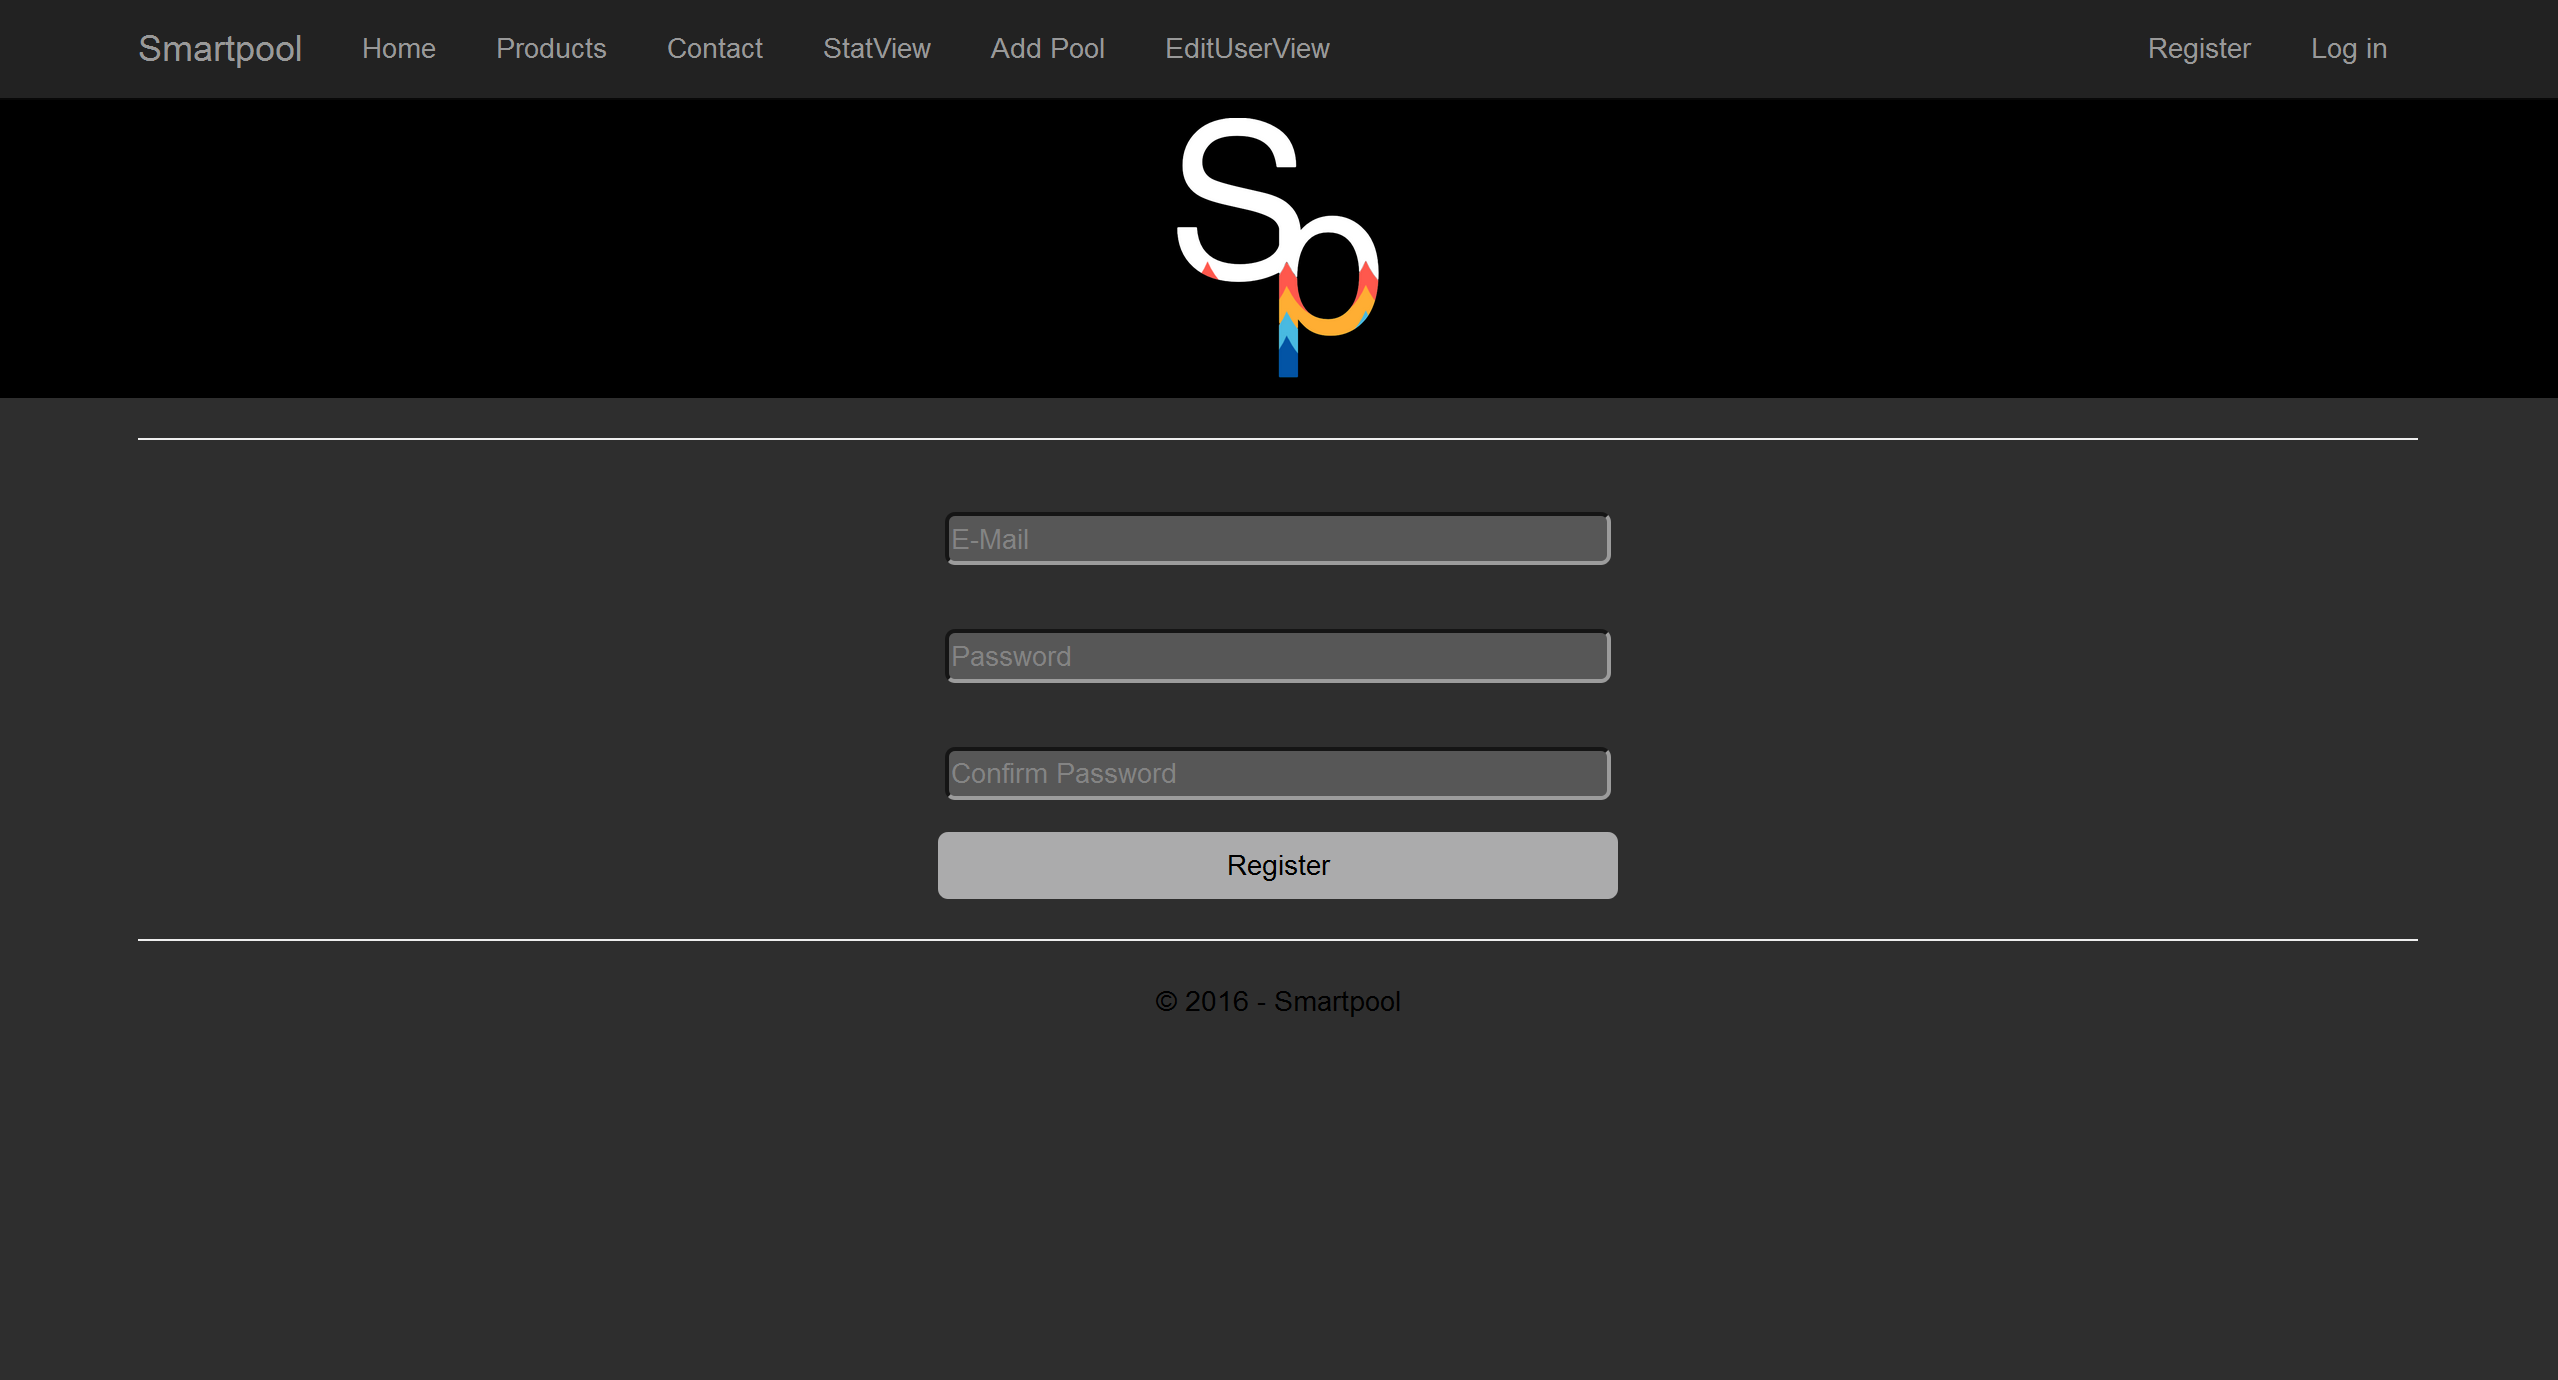
\includegraphics[width=1.0\linewidth]{figs/implementering/web_signupview}
	\caption{Web SignUpView}
	\label{fig:websignupview}
\end{figure}

View grafikken er implementeret jævnfør det grafiske design. AccountController implementerer endnu ikke ISignUpView. Den ene sprint foretaget på Web, havde primært til formål at teste arkitekturen. Grunden tidspres og er implementering af det resterende website blevet nedprioriteret. Det gælder ligeledes for de resterende views.

\subsection{AddPoolView}
AddPoolView ses på figuren nedenfor:

\begin{figure}
	\centering
	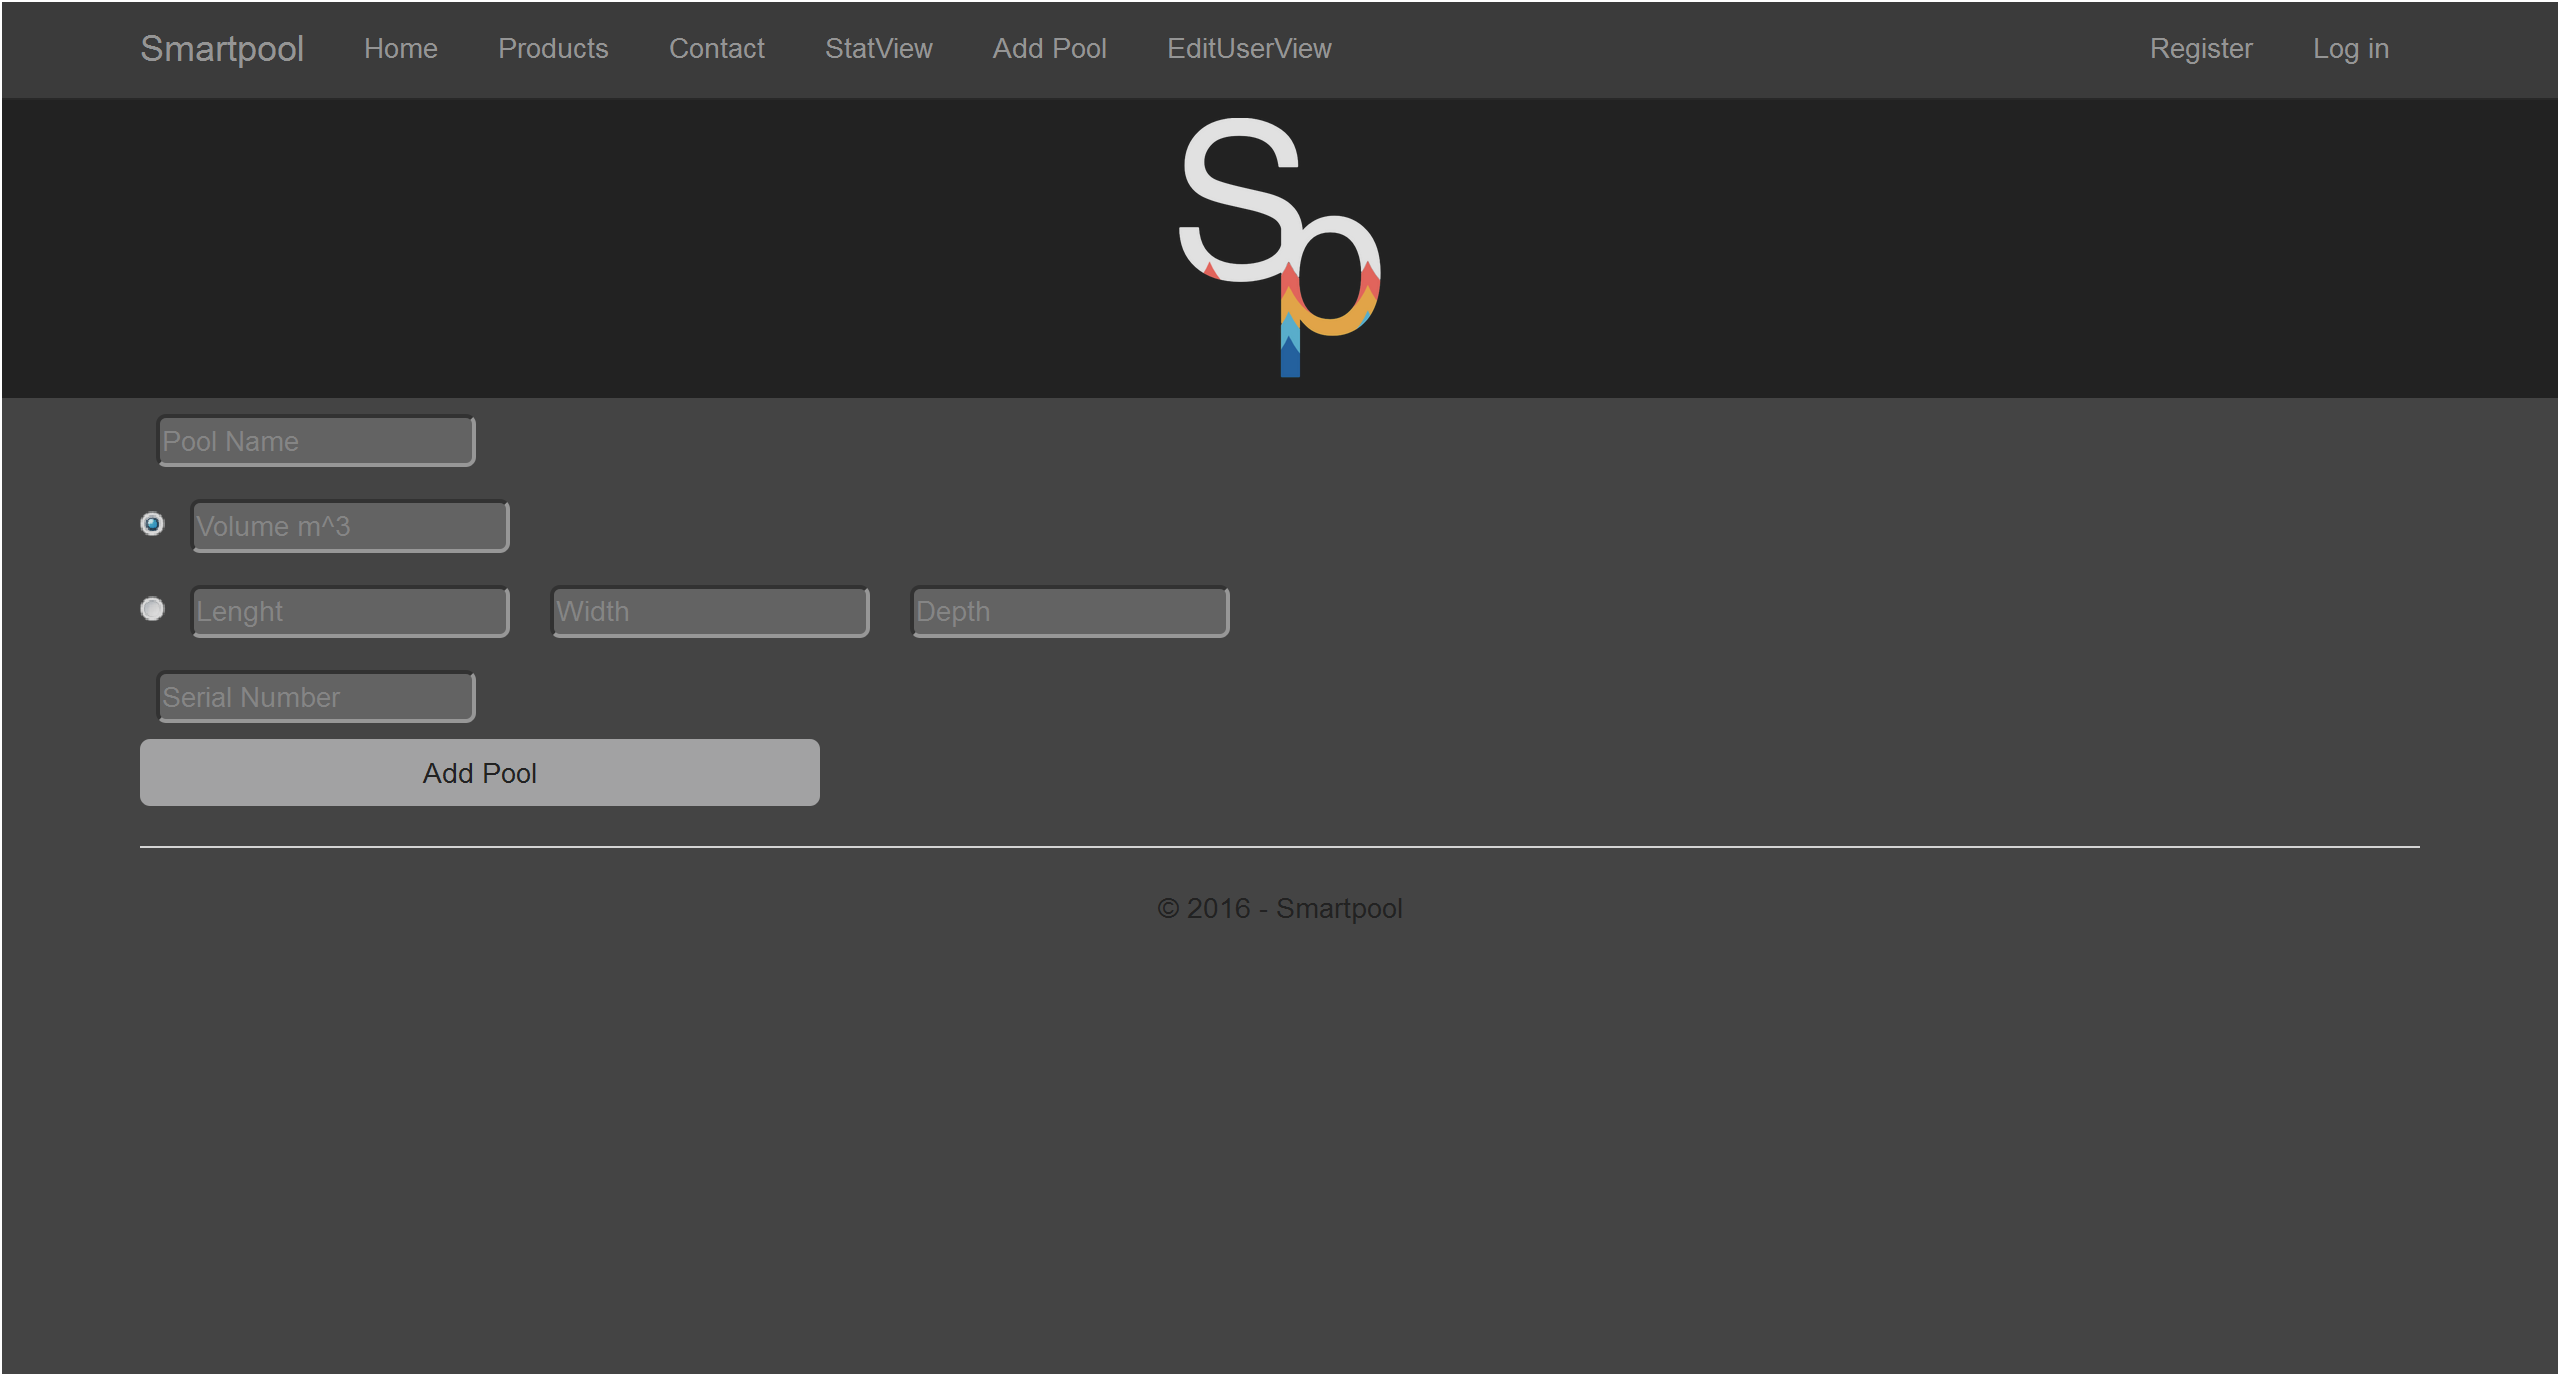
\includegraphics[width=1.0\linewidth]{figs/implementering/web_addpoolview}
	\caption{Web AddPoolView}
	\label{fig:webaddpoolview}
\end{figure}

View grafikken er implementeret jævnfør det grafiske design. AccountController implementerer endnu ikke IAddPoolView. Se \ref{sec: signupview} for yderligere forklaring.

\subsection{EditUserView}
AddPoolView ses på figuren nedenfor:

\begin{figure}
	\centering
	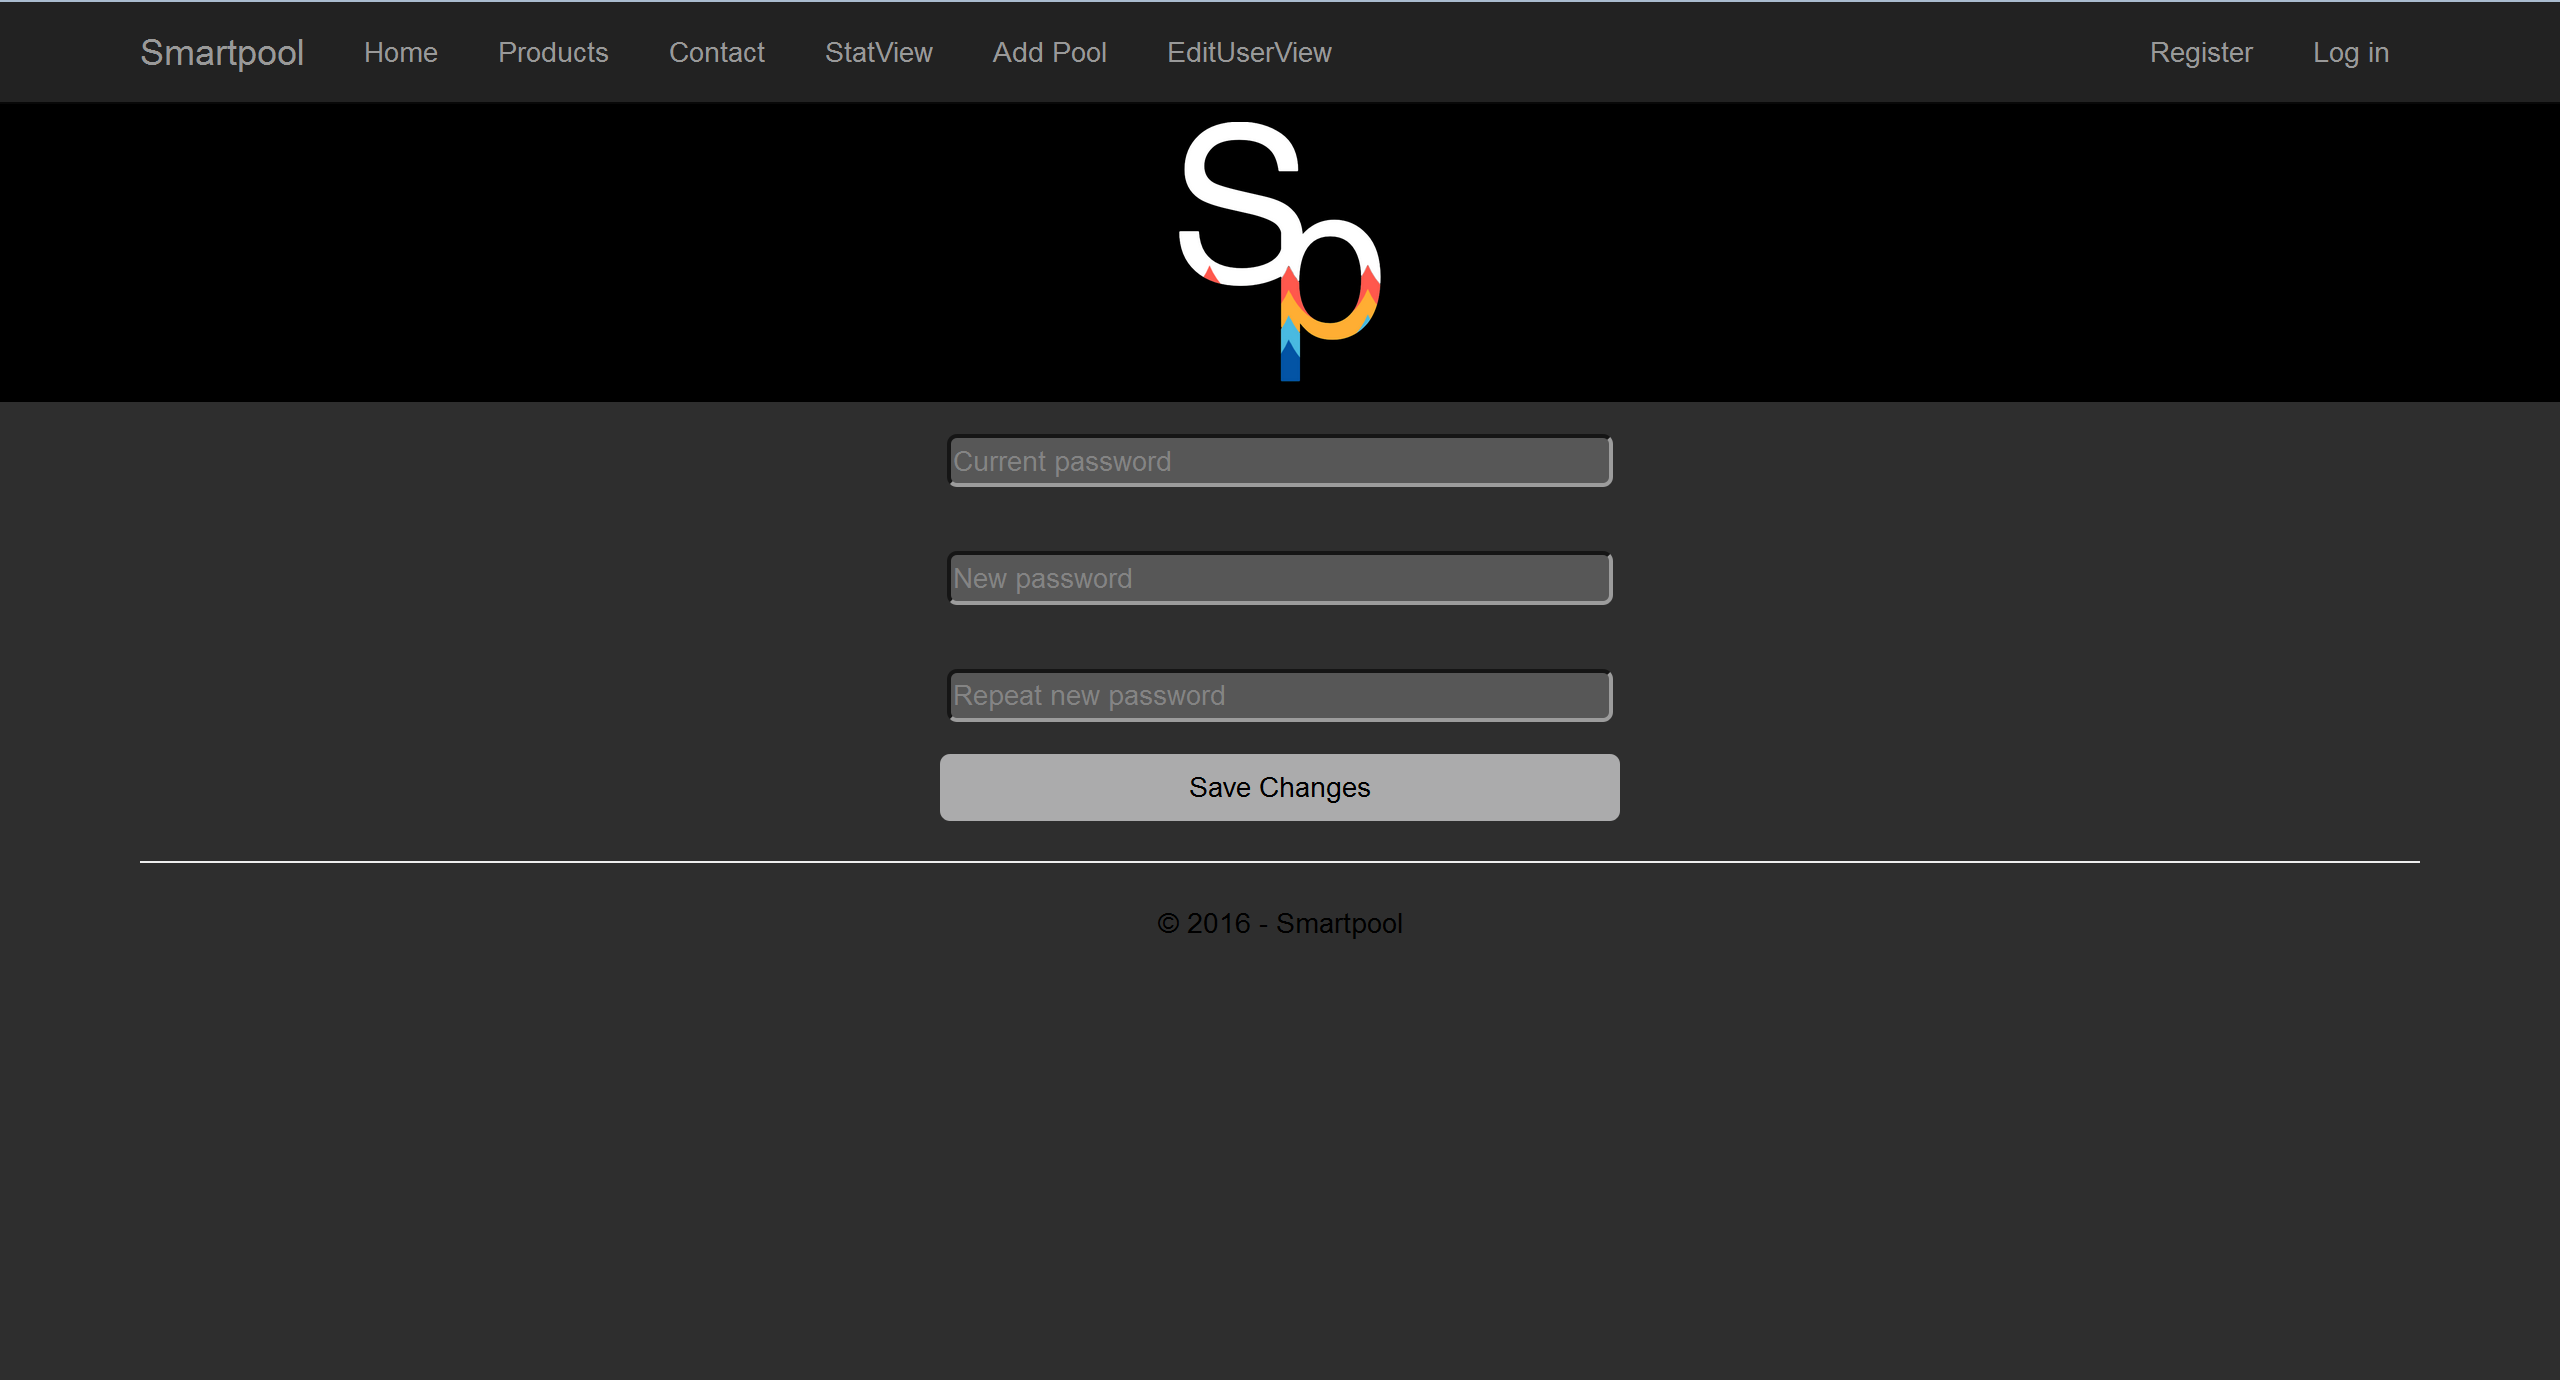
\includegraphics[width=1.0\linewidth]{figs/implementering/web_edituserview}
	\caption{Web EditUserView}
	\label{fig:webedituserview}
\end{figure}

View grafikken er implementeret jævnfør det grafiske design. AccountController implementerer endnu ikke IEditUserView. Se \ref{sec: signupview} for yderligere forklaring.

\subsection{EditPoolView}
Dette view er endnu ikke implementeret. Se \ref{sec: signupview} for yderligere forklaring.

\subsection{StatView}
StatView ses på figuren nedenfor:

\begin{figure}
	\centering
	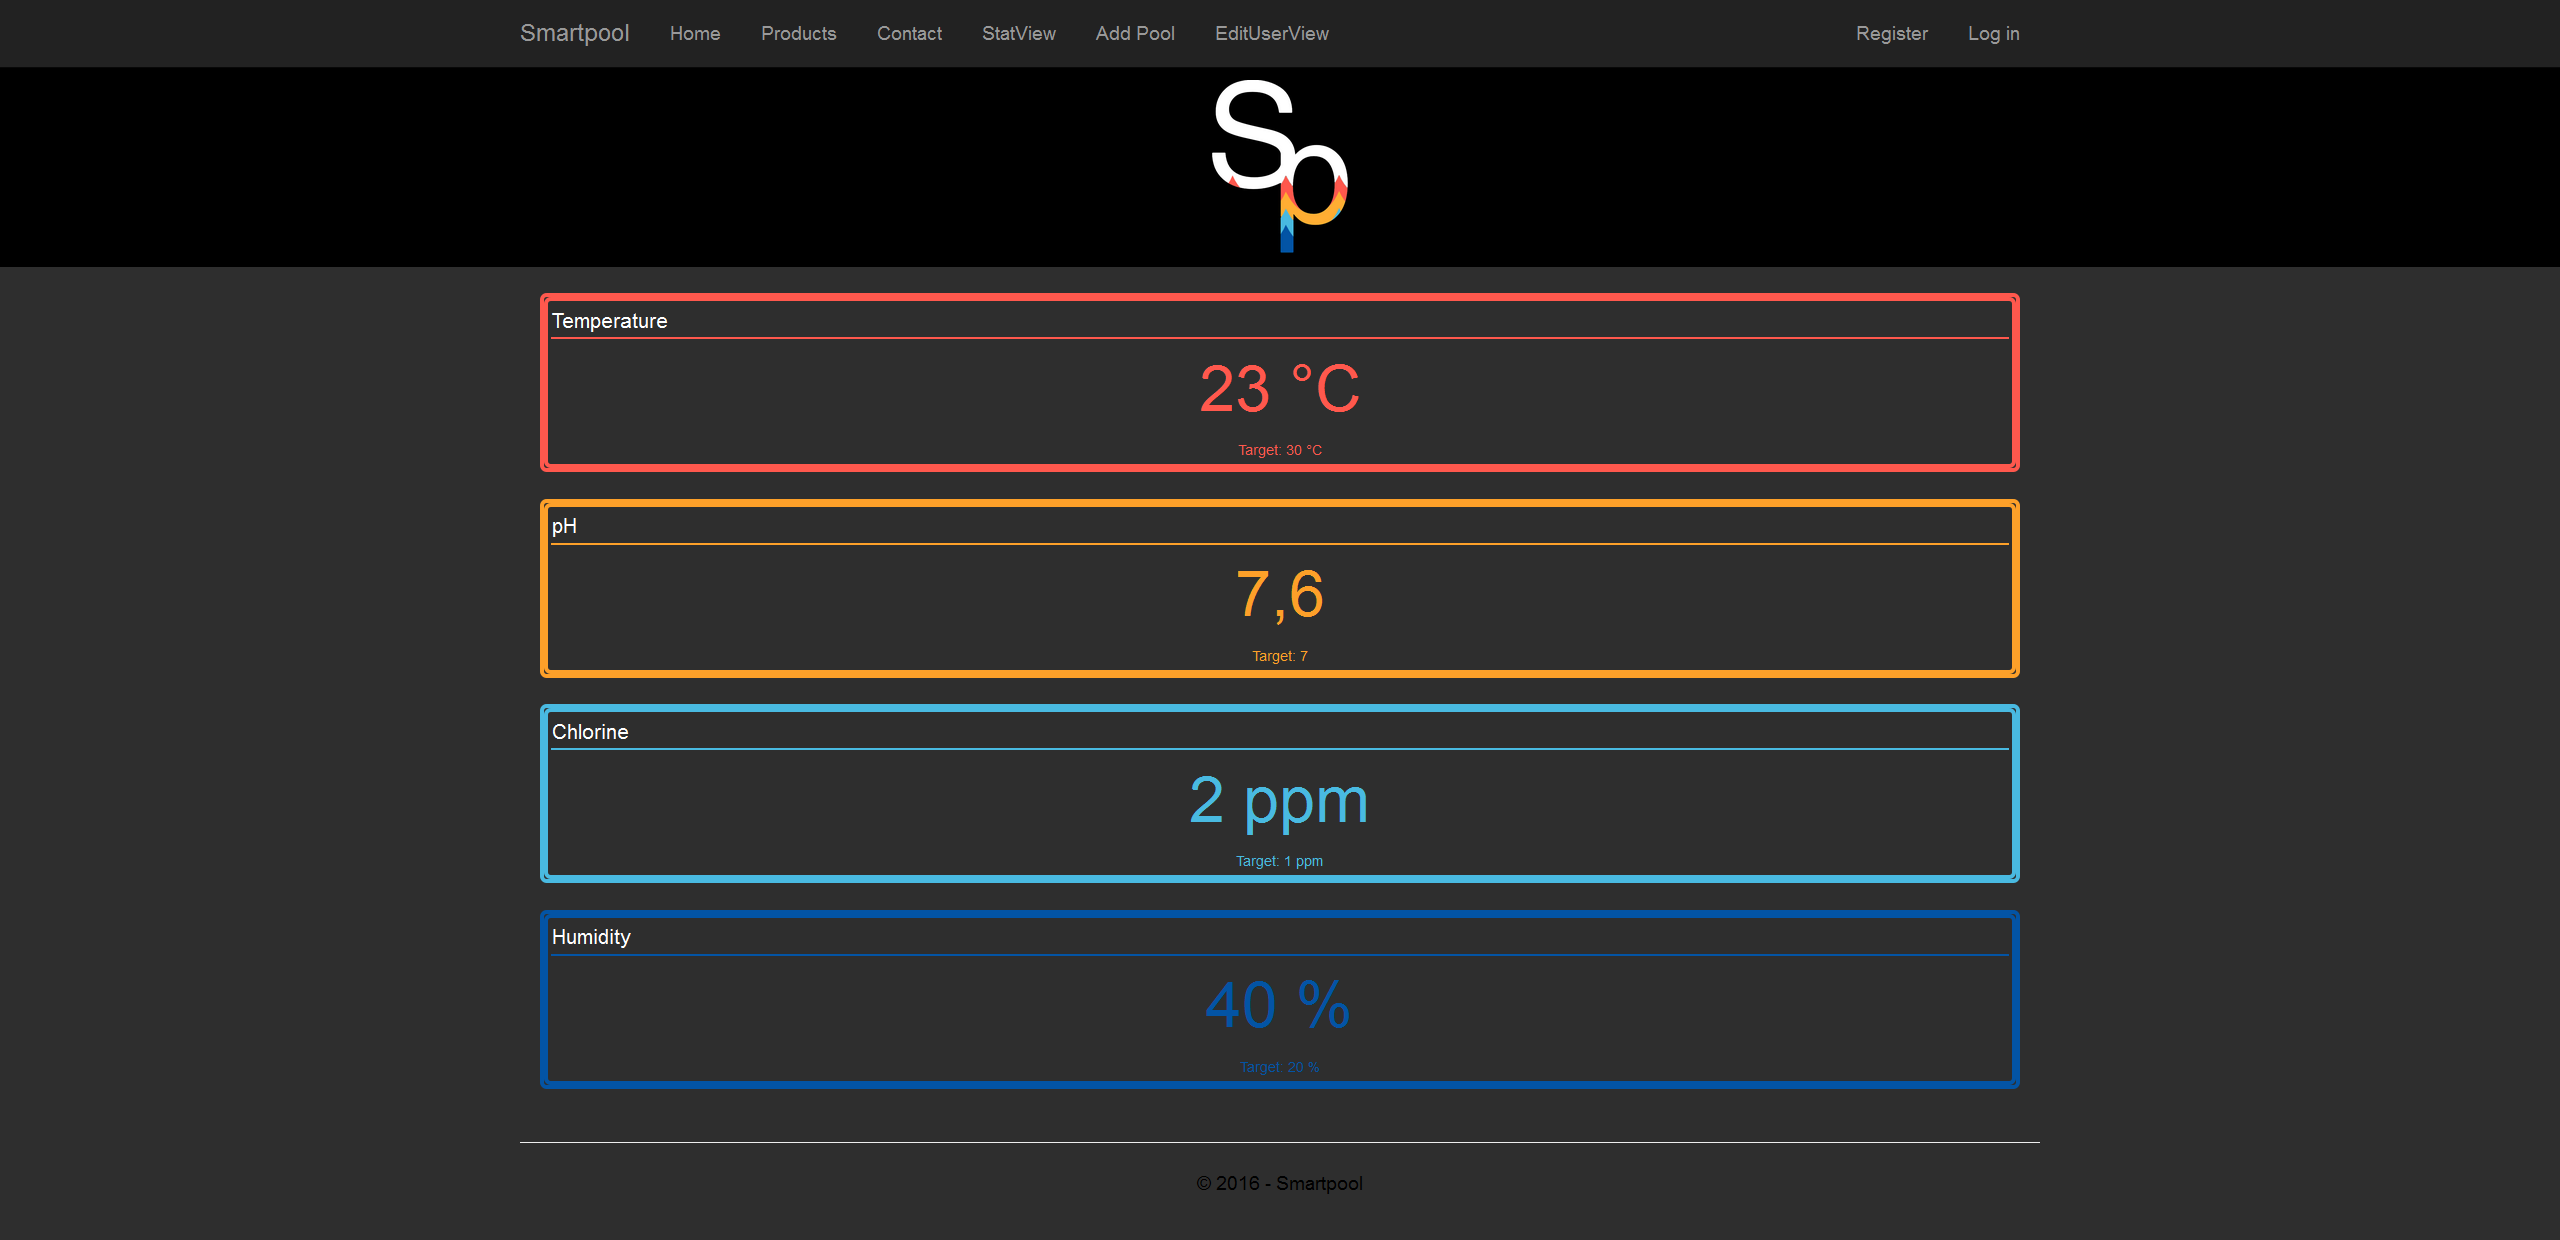
\includegraphics[width=1.0\linewidth]{figs/implementering/web_statview}
	\caption{Web StatView}
	\label{fig:webstatview}
\end{figure}

View grafikken er implementeret jævnfør det grafiske design. AccountController implementerer endnu ikke IStatView. Se \ref{sec: signupview} for yderligere forklaring.

\subsection{HistoryView}

Dette view er endnu ikke implementeret. Se \ref{sec: signupview} for yderligere forklaring.



